% LyX 2.0.5.1 created this file.  For more info, see http://www.lyx.org/.
% Do not edit unless you really know what you are doing.
\documentclass[12pt,english]{report}
\usepackage{mathptmx}
\renewcommand{\familydefault}{\rmdefault}
\usepackage[T1]{fontenc}
\usepackage[latin9]{inputenc}
\usepackage[a4paper]{geometry}
\setcounter{secnumdepth}{2} % Changed from 3 to 2. 0-chapter 1-section 2-subsection 
\setcounter{tocdepth}{2} % Changed from 3 to 2. 0-chapter 1-section 2-subsection 
\setlength{\parskip}{\medskipamount}
\setlength{\parindent}{0pt}
\usepackage{verbatim}
\usepackage{pdfpages}
\usepackage{graphicx}
\usepackage{subfig} %% This package has to be here
\usepackage{setspace}
\usepackage{arabtex}
\usepackage[numbers]{natbib}
\usepackage{nomencl}
\usepackage{amsthm}
\usepackage{amsmath}
\usepackage{amsfonts}
\usepackage{paralist}
\usepackage{etoolbox}
\newtoggle{edit-mode}
\toggletrue{edit-mode}  
%%\toggletrue{edit-mode}
\iftoggle{edit-mode}{
\geometry{verbose,tmargin=2cm,bmargin=2cm,lmargin=2cm,rmargin=6cm,headheight=1cm,headsep=1cm,footskip=1cm, marginparwidth=5cm}
}{
\geometry{verbose,tmargin=2cm,bmargin=2cm,lmargin=2cm,rmargin=2cm,headheight=1cm,headsep=1cm,footskip=1cm}
}

\makenomenclature

%% Theorem Styles
\newtheorem{theorem}{Theorem}[section]
%% Definition Styles
\theoremstyle{definition}
\newtheorem{definition}{Definition}[section]
\newtheorem{example}{Example}[section]
\theoremstyle{remark}
\newtheorem{remark}{Remark}

\usepackage[linesnumbered]{algorithm2e}

\begin{document}

\chapter{Data Collection}
\label{chap:data_collection}

\section{The ADAB Database}
\label{sec:adab_database}

\iftoggle{edit-mode}{\hspace{0pt}\marginpar{The data importance}}{}
The Data, it's quality and quantity, are fundamental aspects of any pattern recognition technique.
It is used for learning, validation and testing stages and has a critical effect on the system accuracy and performance.

\iftoggle{edit-mode}{\hspace{0pt}\marginpar{Data representation Definition}}{}
On-line handwriting data is commonly a digitized representation of the pen movement. 
It may contain sequential information about position, velocity, acceleration, pressure, or even angle and orientation of the pen as a function of time. 
Nevertheless, the most commonly used property is the pen's position. 
Although the sampling of the pen position is done in a constant time intervals, the vast majority of HWR system do not use the temporal information but only consider the ordered set of sequential pen position. 

\iftoggle{edit-mode}{\hspace{0pt}\marginpar{Lack of databases}}{}
Many databases were developed for HWR of English script. 
Among these we can mention the following popular database: UNIPEN, CEDAR, NIST, IRONOFF , etc.
However, very few databases were developed for the Arabic script and fewer became publicly available, such as IFN/ENIT and CEDAR. 
Thus, most researchers had developed their own limited datasets that are not available to the public \cite{saabni2009efficient} 
There is only a single medium size public corpus of on-line Arabic handwriting.
The reason for this lack in database may be attributed to the fact that the major work done on Arabic handwriting recognition, focused on recognizing off-line script \cite{plamondon2000online}. 
Another reason is that most of the work in on-line script recognition field is done for isolated characters such as letters, digits and symbols \cite{al2011online}.

\iftoggle{edit-mode}{\hspace{0pt}\marginpar{Information about the ADAB database}}{}
In this work we have chosen to use the ADAB (Arabic DAtaBase) database.
The ADAB database is de-facto a standard in the on-line Arabic handwriting recognition field.
It was developed to advance the research and development of Arabic on-line handwritten text recognition systems \cite{el2011line}.
It is freely available and consists of more than 20k Arabic handwritten words scribed by more than 170 different writers.
The samples are words that were taken from the 937 Tunisian town/village names, and for this reason, a sample can contain more than a word.
The information saved in the database is the strokes information in an XML file format. 
Each stroke, represented as a node in the XML, contains the sequence of $(x,y)$ coordinates of the pen position expands from the pen-down event to the corresponding pen-up event, as can be seen in Figure \ref{fig:adab_inkml}.
In addition to the strokes positional information, the database contains several properties related to the equipment used to obtain the data and the writer's information, as well as the plot image of the word trajectory as shown in Figure \ref{fig:sample_parts}.

\begin{figure}
\centering
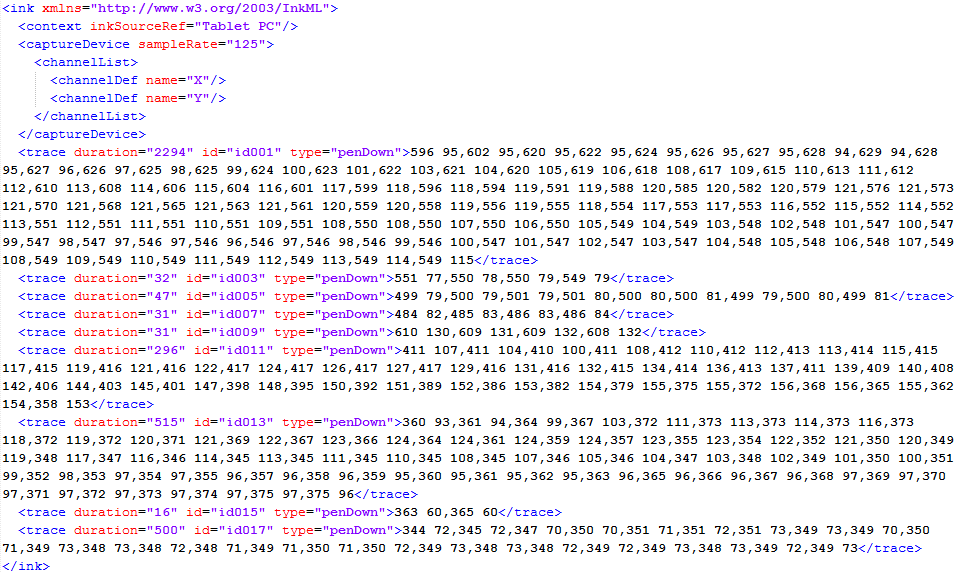
\includegraphics[width=1\textwidth]{./figures/adab_inkml}
\caption{Trajectory information of a city name sample.}
\label{fig:adab_inkml}
\end{figure}

\begin{figure}
\centering
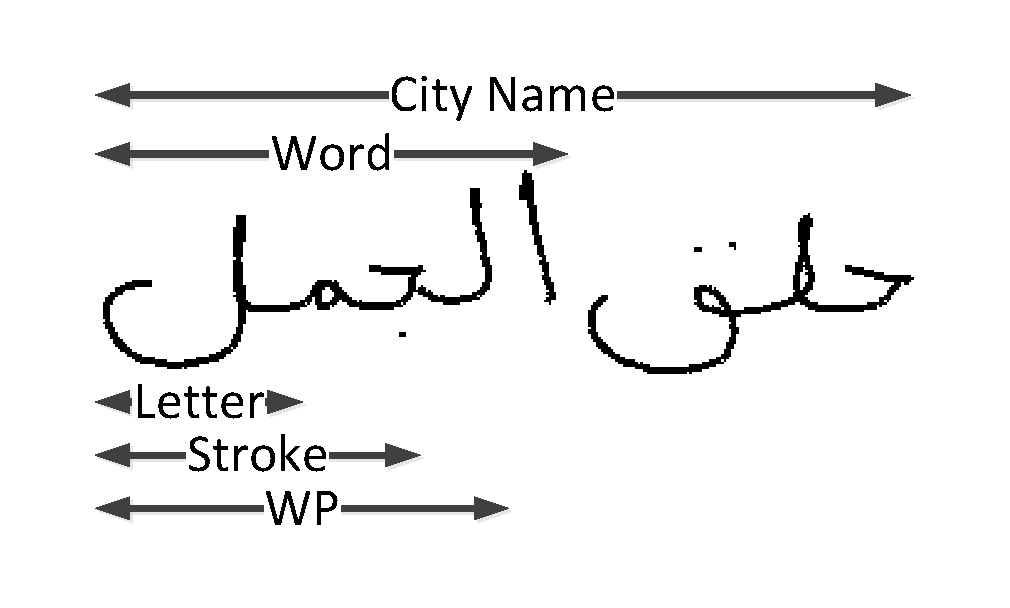
\includegraphics[width=0.65\textwidth]{./figures/sample_parts}
\caption{Visual demonstration of a test sample parts.}
\label{fig:sample_parts}
\end{figure}


%%%%%%%%%%%%%%%%%%%%%%%%%%%%%%%%%%%%%%%%%%%%%%%%%%%%%%%
\newpage{}
%%%%%%%%%%%%%%%%%%%%%%%%%%%%%%%%%%%%%%%%%%%%%%%%%%%%%%%

\section{Letter Samples Extraction}
\label{sec:letters_extraction}

\iftoggle{edit-mode}{\hspace{0pt}\marginpar{The missing information}}{}
The primary task of this stage was to create a sufficiently large database of on-line handwritten Arabic letters to be used by the letter classifier described in Chapter \ref{chap:classification} .
This data, also required for the validation and testing of the system, was extracted by manually the strokes trajectories provided in the ADAB database.
As can be seen in Figure \ref{fig:sample_parts}, the only information provided by the ADAB database is the strokes and their order of writing.
The absence of mapping between the strokes and letters or WP required extra work to add this information to the database so that it could be used as letter samples source and also as a ground-truth for for validating our segmentation algorithm accuracy.
The database construction included semi-manual matching between each strokes and WPs, and then manual segmentation of each stroke. 

\iftoggle{edit-mode}{\hspace{0pt}\marginpar{Letters extraction method}}{}
To ease the tasks mentioned above we've created a user friendly system that reads the samples from the ADAB database, and employs the skills of a human expert to segment the samples and relate each stroke to the corresponding letter in the WP. 
The graphical user interface of the system is shown in Figure \ref{fig:manual_segmentation}. 

\begin{figure}[h]
\centering
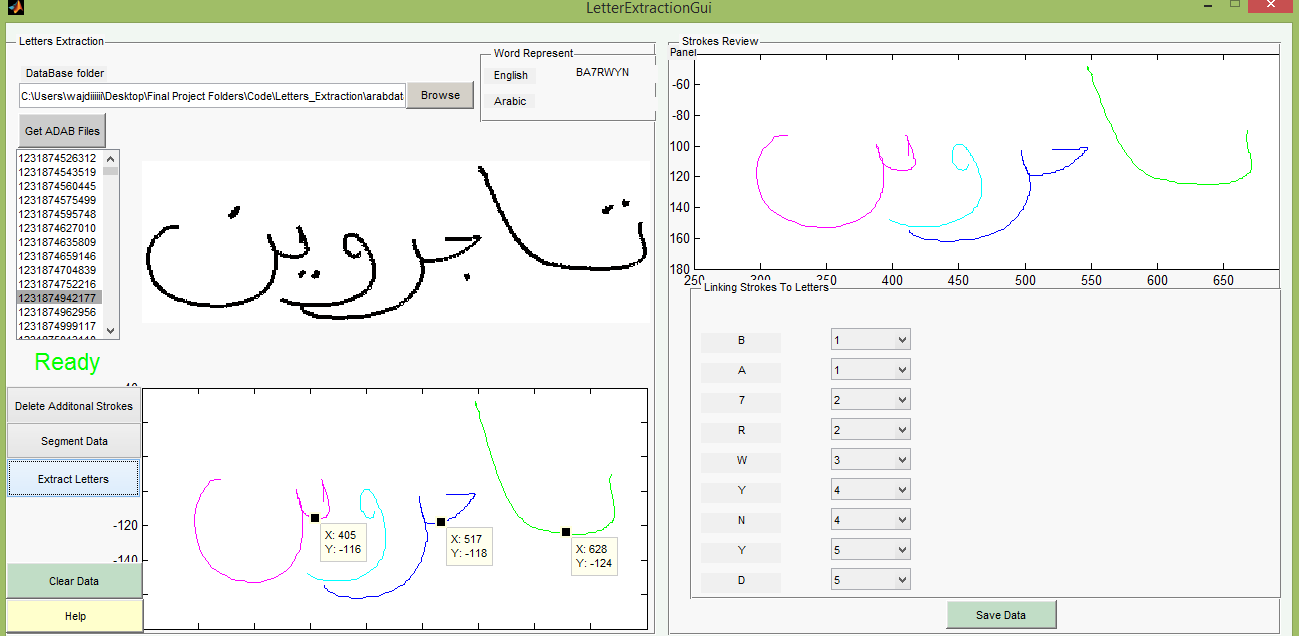
\includegraphics[width=1\textwidth]{./figures/manual_segmentation}
\caption{Manual Segmentation System.}
\label{fig:manual_segmentation}
\end{figure}

\iftoggle{edit-mode}{\hspace{0pt}\marginpar{Additional strokes detection and removal}}{}
Since additional strokes are not our interest in the segmentation process, the system automatically filters out additional strokes. 
The detection of delayed strokes is performed based on their size and the area of their bounding box. 
However, in order to avoid unintentionally removing the main body of small letters, we preset a low high threshold. 
Thus, the human expert had to filter out additional strokes manually that could not be identified by the system as such.

\iftoggle{edit-mode}{\hspace{0pt}\marginpar{The output structure}}{}
The resulted information was saved in an XML file for each word sample. As can be seen in figure \ref{fig:adab_segmented_xml}, the hierarchy of the XML represents the structure of the sample that corresponds to the sample structure as seen in Figure \ref{fig:sample_parts}. 
This XML is used as the ground truth in both learning, testing and validation processes.
In order to obtain a sufficient size sample set for both learning and validation, more than 16k samples were manually segmented which consisted of about 40k letters. 

\begin{figure}
\centering
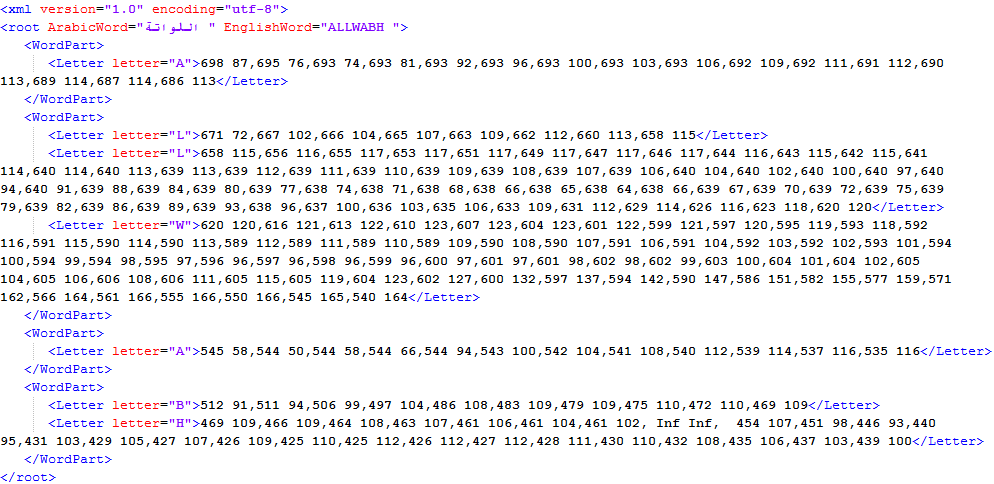
\includegraphics[width=1\textwidth]{./figures/adab_segmented_xml}
\caption{Trajectory information of a city name sample.}
\label{fig:adab_segmented_xml}
\end{figure}

\bibliographystyle{plainnat}
\bibliography{references}
\end{document}

%\begin{itemize}
%\item mention that the number of samples per class is different from letter to letter
%\item see "Removing delayed strokes" section in \cite{jaeger2001online}
%\end{itemize}
